\documentclass[a4paper,11pt]{article}
\usepackage[T1]{fontenc}
\usepackage[utf8]{inputenc}
\usepackage{lmodern}

\usepackage{amsmath}
\usepackage{amsthm}

\usepackage{graphicx}
\graphicspath{{../data/}}
\usepackage{caption}

\usepackage{fullpage}

\renewcommand{\thesubsection}{\alph{subsection}}

\newcommand{\pitem}[2]{
\item
\begin{tabular*}{3in}{p{1in}p{1.2in}}
		#1 & \hfill #2 \\
\end{tabular*}\vspace{-6pt}}

\usepackage{qtree}

\title{Image Processing 1 - Exercise 6 - WiSe 2012/13}
\author{Weipeng He \\ \texttt{2he@informatik.uni-hamburg.de} \\ \texttt{6411529}}

\begin{document}

\maketitle

\section{}

\subsection{}
The probability of a pixel to be one of the following is :
\begin{itemize}
  \pitem{background}{$.9$}
  \pitem{black}{\quad $.1 \times .8 = .08$}
  \pitem{yellow}{\quad $.1 \times .01 = .001$}
  \pitem{blue}{\quad $.1 \times .12 = .012$}
  \pitem{red}{\quad $.1 \times .05 = .005$}
  \pitem{green}{\quad $.1 \times .02 = .002$}
\end{itemize}
Therefore, the entropy of the documents would be :
\begin{align*}
  H &= \sum P(g) log_2 \frac{1}{P(g)} \\
    &= .9 \times log_2 \frac{1}{.9} + .08 \times log_2 \frac{1}{.08} + .001 \times log_2 \frac{1}{.001} + .012 \times log_2 \frac{1}{.012} \\
& \qquad + .005 \times log_2 \frac{1}{.005} + .002 \times log_2 \frac{1}{.002} \\
    &= 0.57100
\end{align*}

\subsection{}
Design the Huffman code according to the Huffan code tree shown below :

\Tree [ . [ .0 [ .0 [ .0 [ .0 [ .0 yellow ] [ .1 green ] ] [ .1 red ] ] [ .1 blue ] ] [ .1 black ] ] [ .1 background ] ] 

Thus the codes for each pixel should be :
\begin{itemize}
  \pitem{background}{\texttt{1}}
  \pitem{black}{\texttt{01}}
  \pitem{yellow}{\texttt{00000}}
  \pitem{blue}{\texttt{001}}
  \pitem{red}{\texttt{0001}}
  \pitem{green}{\texttt{00001}}
\end{itemize}

\subsection{}
The average code word length is
\begin{align*}
  \bar{L} &= .9 \times 1 + .08 \times 2 + .001 \times 5 + .012 \times 3 + .005 \times 4 + .002 \times 5 \\
    &= 1.1310
\end{align*}

\subsection{}
The redundancy of the 4-bit-code is
\[ 4 - H = 3.4290 \]

\section{}
Source code can be found in \texttt{src/segment.py}.

Original and segmented picture are as shown below:

\begin{center}
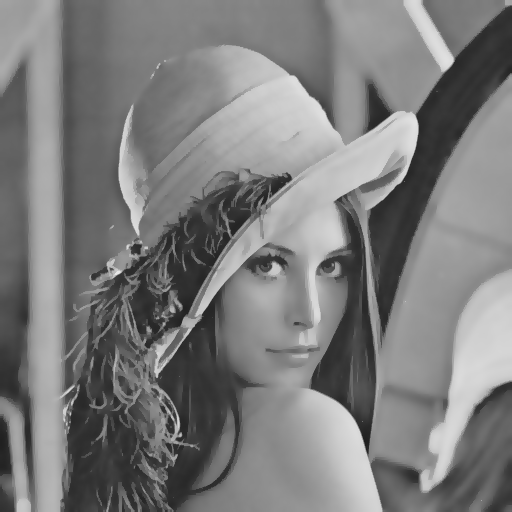
\includegraphics[width=.5\textwidth]{lenna}

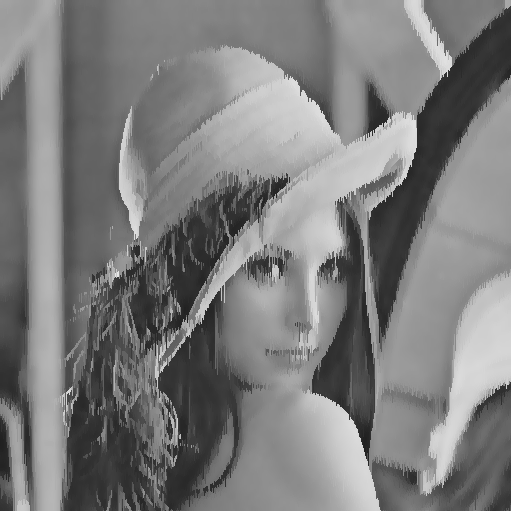
\includegraphics[width=.5\textwidth]{segment}
\end{center}


\end{document}
